\documentclass[a4paper,10pt,oneside]{article}
\usepackage{graphicx}
\usepackage{color}
\usepackage{url}
\usepackage{subfigure}
\usepackage[utf8]{inputenc}
\usepackage[T1]{fontenc}
\usepackage{tgpagella}
%\usepackage[scale=0.9]{tgcursor}
%\usepackage[scale=0.9]{tgheros}
\usepackage{xstring}
\usepackage{wrapfig}

\newcommand{\myscale}{0.74}
\newcommand{\vect}[1]{\boldsymbol{#1}}
\newcommand{\code}[1]{\texttt{\StrSubstitute{#1}{.}{.\.}}}
\def\.{\discretionary{}{}{}}
\newcommand{\jmodule}[1]{\texttt{\textit{#1}}}

\setlength{\hoffset}{-1in} %left margin will be 0, as hoffset is by default 1inch
\setlength{\voffset}{-1in} %analogous voffset
\setlength{\oddsidemargin}{1.5cm}
\setlength{\evensidemargin}{1.5cm}
\setlength{\topmargin}{1.5cm}
\setlength{\textheight}{24cm}
\setlength{\textwidth}{18cm}

\def\mftitle{jInfer TwoStepSimplifier Module Description}
\def\mfauthor{Michal Klempa, Mário Mikula, Robert Smetana, Michal Švirec, Matej Vitásek}
\def\mfadvisor{RNDr. Irena Mlýnková, Ph.D., Martin Nečaský, Ph.D.}
\def\mfplacedate{Praha, 2011}
\title{\bf\mftitle}
\author{\mfauthor \\ Advisors: \mfadvisor}
\date{\mfplacedate}

\ifx\pdfoutput\undefined\relax\else\pdfinfo{ /Title (\mftitle) /Author (\mfauthor) /Creator (PDFLaTeX) } \fi

\begin{document}
\maketitle
\noindent Target audience: developers willing to extend jInfer, scientist willing to implement own inference methods

\noindent \emph{Note: we use the term \textbf{inference} for the act of creation of schema throughout this and other jInfer documents.}

\noindent \begin{tabular}{|l|l|} \hline
Responsible developer: & Michal Klempa \\ \hline
Required tokens:       & cz.cuni.mff.ksi.jinfer.base.interfaces.RuleDisplayer \\ \hline
Provided tokens:       & cz.cuni.mff.ksi.jinfer.base.interfaces.inference.Simplifier \\ \hline
Module dependencies:   & AutoEditor, Base, JUNG, Lookup \\ \hline
Public packages:       & \\ \hline
\end{tabular}

%#### INTRO ############################################
\section{Introduction}
With \jmodule{TwoStepSimplifier} we provide user a complex solution of grammar inference problem.
This is the only one simplifier shipped with jInfer, but it has many features and replaceable submodules of which we implement alternatives in basic bundle.
We implement is $k,h$-context method of infering grammar rules (see \cite{ahonen}).
This process is split into submodules with generic automaton implementation, so it is easy to plug-in any other automaton merging state algorithm.
In this document, we will walk over all modules and submodules in simplifier and describe them briefly.

%#### FACTORY ############################################
\section{Using of factory pattern} \label{section_factory}
Lets stay a while at factory pattern usage.
In \jmodule{TwoStepSimplifier} we employ factory pattern (as described in \cite[section 4.2]{archdoc}) to divide module into submodules.
Since service providing classes kept singletons, we make them factories:
For example:
\begin{verbatim}
@ServiceProvider(service = AutomatonSimplifierFactory.class)
public interface AutomatonSimplifierFactory extends 
                     NamedModule, Capabilities, UserModuleDescription {
  <T> AutomatonSimplifier<T> create();
}
\end{verbatim}
The real submodule interface (called familiarly \emph{worker} interface) is the \code{AutomatonSimplifier<T>} interface (of which instance is returned by factory).
It is now not important how worker interface looks like, lets examine the factory.

In \jmodule{Two\.Step\.Sim\.pli\.fier} we design service providing factory interfaces so that they extend \code{Na\.med\.Mo\.du\.le}, \code{Ca\.pa\.bi\.li\.ties} and \code{UserModuleDescription}.
That means, modules must implement methods:
\begin{verbatim}
String getName();
String getDisplayName();
String getModuleDescription();
List<String> getCapabilities();
String getUserModuleDescription();
\end{verbatim}
Nothing non-standard, but \code{getUserModuleDescription}.
It returns description of the module, comprehensive to user, which is then displayed in properties panels.

In some circumstances, it is useful to declare method \code{create()} generic.
The \jmodule{AutomatonSimplifier} works with \code{Automaton} instances, which themself are generic, too.
But simplifying of automaton does not depend on type of symbol of automaton transitions, so interface \code{AutomatonSimplifier<T>}
is also generic.
Factory interface deals with this by defining \code{create()} method generic, too.

Our usage of this factory pattern follows the routine:
\begin{verbatim}
final Properties p = RunningProject.getActiveProjectProps(getName());

AutomatonSimplifierFactory f = ModuleSelectionHelper.lookupImpl(AutomatonSimplifierFactory.class,
   p.getProperty(PROPERTIES_AUTOMATON_SIMPLIFIER));

AutomatonSimplifier<AbstractStructuralNode> autSmp = f.<AbstractStructuralNode>create();
...
result= autSmp.simplify(something_to_process);
\end{verbatim}
If one module has some submodules, we implement lookups for submodule implementations in our own factory \code{create} method.
Worker class receives factories of all of its submodules as a constructor parameters.

Lets look on \code{AutomatonMergingStateFactory}, that is factory of module, which has \jmodule{AutomatonSimplifier} as a submodule.
Its create method is (shortened): 
\begin{verbatim}
@Override
public ClusterProcessor<AbstractStructuralNode> create() {
  LOG.debug("Creating new ClusterProcessorAutomatonMergingState.");
  return new AutomatonMergingState(getAutomatonSimplifierFactory(),
                                   getRegexpAutomatonSimplifierFactory());
}
\end{verbatim}
Methods \code{getAutomatonSimplifierFactory} and \code{getRegexpAutomatonSimplifierFactory} are analogical, we show you the former one:
\begin{verbatim}
private AutomatonSimplifierFactory getAutomatonSimplifierFactory() {
  final Properties p = RunningProject.getActiveProjectProps(getName());

  return ModuleSelectionHelper.lookupImpl(AutomatonSimplifierFactory.class,
            p.getProperty(PROPERTIES_AUTOMATON_SIMPLIFIER,
                          PROPERTIES_AUTOMATON_SIMPLIFIER_DEFAULT));
}
\end{verbatim}
Cluster processor \code{AutomatonMergingState} then receives factories of \jmodule{AutomatonSimplifier} and \jmodule{Reg\.exp\.Au\.to\.ma\.ton\.Simplifier} submodules in its constructor.
Cluster processor then may create as many instances of submodule classes as it needs (maybe simplifying more than one automaton).
Thorough this document, we will mention only worker interface when describing submodule, since all factory interfaces are designed same way, we've just described.


%#### STRUCTURE ############################################
\section{Structure}
\jmodule{TwoStepSimplifier} is implemented in package \code{cz.cuni.mff.ksi.jinfer.twostep}.
Module is divided into two classes: \code{TwoStepSimplifier} (main logic), \code{TwoStepSimplifierFactory} (lookups, interface to other modules).
Latter one is registered as service provider (and implements) of \code{Simplifier} interface (defined in package \code{cz.cuni.mff.ksi.jinfer.base.interfaces.inference}).

It has main method called \code{start} which receives Initial Grammar in form of
\begin{verbatim}
final List<Element> grammar
\end{verbatim}
Each grammar rule is represented as class \code{Element}, where element is left side of rule and it's \code{getSubnodes()} method
returns regular expression, which is right side of rule (as described in \cite[3.1.1]{archdoc}, they are all concatenations).
Second parameter is 
\begin{verbatim}
final SimplifierCallback callback
\end{verbatim}
Callback which should be called when work is done.
On output, simplifier provides Simplified grammar as a parameter into callback function:
\begin{verbatim}
void finished(final List<Element> grammar);
\end{verbatim}
Thus simplifier receives Initial Grammar and returns Simplified grammar, both represented same way - list of elements.

\code{TwoStepSimplifierFactory.start()} creates new \code{TwoStepSimplifier} class instance, providing three factories of submodules to its constructor.
Then it calls \code{simplify(initialGrammar)} method of this instance and its result passes as parameter to callback function.
Thats all, the magic comes in \code{TwoStepSimplifierFactory} class.

\section{Modular design}
\jmodule{TwoStepSimplifier} is inspired by \cite{1802522} design. Inference proceeds in two steps:
\begin{enumerate}
	\item clustering of element instances into clusters of (probably) same elements
	\item infering regular expression for each element from examples of element contents taken from all elements in cluster
\end{enumerate}
Task of clustering is dedicated to \jmodule{Clusterer} submodule, and task of infering regular expression for each cluster is dedicated to \jmodule{ClusterProcessor} submodule. We will examine both of them.
There is also third submodule called \jmodule{RegularExpressionCleaner} actually, its purpose is just to beautify
 output regular expressions, no inference logic is implemented there. 
Modules are drawn on fig. \ref{twostep_modules}.
\begin{figure}[tpb]
	\centering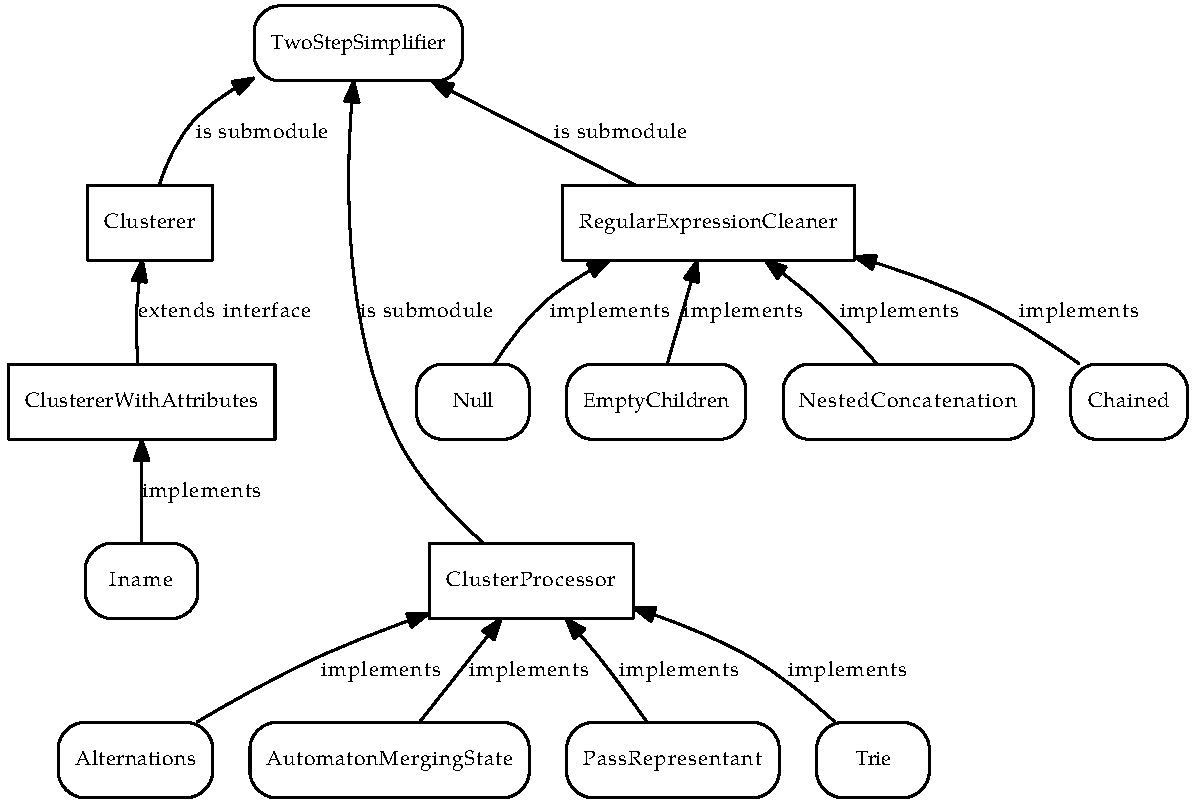
\includegraphics[scale=\myscale]{twostep_modules}
	\caption{Submodules of TwoStep simplifier with their implementations} \label{twostep_modules}
\end{figure}
We provide one \jmodule{Clusterer}, 4 \jmodule{ClusterProcessor} and 4 \jmodule{RegularExpressionCleaner} implementations.
Each of those will be explained further in this document.

Method \code{TwoStepSimplifier.simplify()} does basically this:
\begin{verbatim}
// 1. cluster elements
final Clusterer<AbstractStructuralNode> clusterer= clustererFactory.create();
clusterer.addAll(initialGrammar);
clusterer.cluster();

// 2. prepare emtpy final grammar
final List<Element> finalGrammar= new LinkedList<Element>();

// 3. process rules
final ClusterProcessor<AbstractStructuralNode> processor =
             clusterProcessorFactory.create();
             
for (Cluster<AbstractStructuralNode> cluster : clusterer.getClusters()) {
  final AbstractStructuralNode node =  
                          processor.processCluster(clusterer, cluster.getMembers());
  final RegularExpressionCleaner<AbstractStructuralNode> cleaner = 
                          regularExpressionCleanerFactory.<AbstractStructuralNode>create();
  // 4. add to rules
  finalGrammar.add(
              new Element(node.getContext(),
              node.getName(),
              node.getMetadata(),
              cleaner.cleanRegularExpression(((Element) node).getSubnodes()),
              attList));
}

return finalGrammar;
\end{verbatim}
It creates clusterer, gives it all rules, orders it to cluster elements.
Then, empty list of elements is created as final (simplified) grammar.
For each input rule in \code{initialGrammar}, submodule \jmodule{ClusterProcessor} is called to do infering of regular expression of that element.
Finally, regular expression cleaning is done in submodule and new \code{Element} instance is created as a copy of processed node, but with infered and cleaned regexp.

\paragraph{Sentinel processing}
There are some specialities in processing sentinel elements (see \cite[3.2]{archdoc}).
Sentinels can be only on right side of rules and they have to be send to clusterer, as someone further in the chain can ask for cluster of sentinel element - which appears on right side.
But sentinels have no content, they must not be taken into account when infering attribute properties (whether it is required or optional) - since sentinel have no attributes at all.

Now we will examine submodules for clustering, processing and cleaning.


%#### STRUCTURE->Clusterer ############################################
\subsection{Clusterer submodule}
We implement clustering in \code{cz.cuni.mff.ksi.jinfer.twostep.clustering} package.
One cluster is represented by class \code{Cluster<T>} with \code{T} as type of clustered items.
This class simply holds java set of members of cluster and one of the references is held also in \code{representant} member.

We provide \code{Clusterer} interface for classes to implement.
Its purpose is to cluster bunch of elements (rules) on input, into  bunch of \code{Cluster} class instances (cluters) on output.
It has methods \code{add()} and \code{addAll()} for adding items for clustering.
Centerpart is method \code{cluster()}, which does the clustering itself.

As it may be time-consuming operation, method throws \code{InterruptedException}.
Implementation should take care of checking whether thread is user interrupted (see \cite[p. 12]{archdoc}).
After clustering, implementation should hold clusters in member, as it will be later requested by calling method \code{T getRepresentantForItem(T item)}.
Given item to this method, one can ask for representant of cluster, to which the item belongs.
If no such cluster exists (item was not added for clustering before), we recommend you throwing an exception rather than returning \code{null}.
Missing item will probably  indicate error in algorithm rather than normal workflow.
One can pull clusters (\code{List<Cluster<T>{}>}) from clusterer by calling \code{getClusters()} method.
Basic work usage with clusterer is:
\begin{verbatim}
Clusterer <T> c = new MyContextClusterer<T>();
c.addAll(initialGrammar);
c.cluster();
...
c.getClusters();
or
c.getRepresentantForItem(x);
\end{verbatim}

%#### STRUCTURE->Clusterer->WithAttributes ############################################
\subsubsection{ClustererWithAttributes extended interface}
You noticed that whole \jmodule{Clusterer} interface and \code{Cluster} class are generic.
They may be used as design pattern not only for clustering elements in inference process.
To address clustering of elements in more detail, we created \code{Cluster\.er\.With\.At\.tri\.bu\.tes<T, S>} interface, which extends \code{Clusterer<T>} interface.
It adds method \code{List\.<Cluster<S>{}> get\.At\.tri\.bu\.teClusters(T representant)}, implying that each representant of
type \code{T} (that is representant of some main cluster) has some "attribute" clusters associated with it.
Attribute clusters are of type \code{S} and can be retrieved by calling \code{getAttributeClusters(x)}.

We provide one implementation of this interface described in \ref{section_Iname}.

%#### STRUCTURE->ClusterProcessor ############################################
\subsection{ClusterProcessor module}
\jmodule{ClusterProcessor} takes rules of one cluster of element and somehow obtains regular expression for that set of elements. It returns one rule - element with name set to desired name of element in schema (not all elements in cluster have to have same name, if advanced clustering scheme is used, then processor has to choose right name for the resulting element) and with subnodes set to regular expression infered.
It process attributes of all elements in cluster to obtain meaningful schema attribute specification and theese attributes has to attach to the resulting element.

Worker interface itself is defined as follows:
\begin{verbatim}
public interface ClusterProcessor<T> {
  T processCluster(
          final Clusterer<T> clusterer,
          final List<T> rules
          ) throws InterruptedException;
}
\end{verbatim}
Why cluster processor is given the clusterer instance?
Rules themself contain information about which elements to process, but clusterer has more information
about the topic.
Clusterer can tell you representant for any element in whole input (not only those elements in rules, but also those that may be on right side of rules), clusterer (if it is with attributes) has information about attributes of each cluster.

We describe each \jmodule{ClusterProcessor} implementation we've got in sections \ref{section_PassRepresentant} through \ref{section_AutomatonMergingState}.

%#### STRUCTURE->RegularExpressionCleaner ############################################
\subsection{RegularExpressionCleaner module}
Last we examine \jmodule{RegularExpressionCleaner} interface.
Purpose of this submodule is only to make output regular expression corrections, to make them nicer.
For example it is common that converting automaton to regular expression by state elimination produces nested concatenations such like $(name, (person, id))$.
To convert such expression into $(name, person, id)$, one can implement this interface and connect it to work in chain.
Interface is definition is straightforward:
\begin{verbatim}
public interface RegularExpressionCleaner<T> {
  Regexp<T> cleanRegularExpression(final Regexp<T> regexp);
}
\end{verbatim}
Given regular expression, return regular expression.
Converting of regular expression is commonly a recursive task and all our implementations work this way.

%#### PREFERENCES ############################################
\section{Preferences}
All settings provided by \jmodule{TwoStepSimplifier} are project-wide, the preferences panel is in \code{cz.cuni.mff.ksi.jinfer.twostep.properties} package.
It is possible to:
\begin{itemize}
	\item select \jmodule{Clusterer} submodule implementation from those installed
	\item select \jmodule{ClusterProcessor} submodule implementation from those installed
	\item select \jmodule{RegularExpressionCleaner} submodule implementation from those installed
\end{itemize}

%#### DATA FLOW ############################################
\section{Data flow}
\begin{figure}[tpb]
	\centering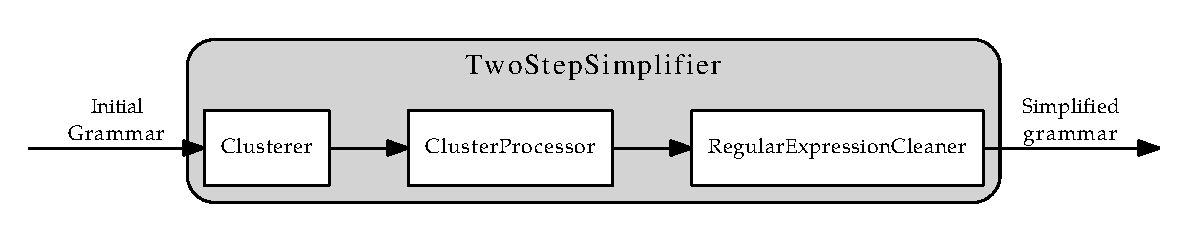
\includegraphics[scale=1]{twostep_flow}
	\caption{TwoStep data flow} \label{twostep_flow}
\end{figure}
Process illustrated on fig. \ref{twostep_flow}:
\begin{enumerate}
	\item On input there is Initial Grammar, which is ruled into \jmodule{Clusterer}.
	\item Then, each cluster is sent to submodule \jmodule{ClusterProcessor}, which returns regular expression for that cluster.
	\item Regular expression is sent to \jmodule{RegularExpressionCleaner} submodule for cleaning.
	\item From each cluster processing, regular expression is added to the list of simplified grammar rules.
	\item List of simplified rules is returned (Simplified grammar).
\end{enumerate}

%#### SUBMODULES ############################################
\section{Submodules implementations}
%#### SUBMODULES->Iname ############################################
\subsection{Iname (ClusteterWithAttributes)} \label{section_Iname}
We cluster elements in \code{Iname<AbstractStructuralNode, Attribute>} class, which takes \code{AbstractStructuralNode} classes to cluster as main, and \code{Attribute} classes as attributes.
Clustering is done based on elements \code{getName} equality test (ignore case).
For each rule (element), it is first clustered by finding cluster where representant has same name - or create new cluster with this element as representant.
Then we process right side of this element rule (that are nodes from \code{getSubnodes}).
Since right side of rule is always concatenation, we simply take \code{.getSubnodes().getTokens()} list and iterate through it.
Each node on right side, is examined:
\begin{itemize}
  \item if it is simple data throw it to \code{SimpleDataClusterer} class which is associated with main element cluster. It does nothing more, than holds all \code{SimpleData} instances in one cluster. But in future it may be replaced to cluster simple data somehow, to obtain meaningful content models in schemas.
  \item if it is element and it is tagged as sentinel by metada - search main clusters to find cluster with representant of same \code{getName()}, or create new cluster with this sentinel as representant. From IGG, sentinels may be only on right sides of rules and since each element in schemas has to be defined, there must exist another element with same name, which is not sentinel (and maybe it will come to process in future). So there can't be cluster with only one sentinel element in it.
  \item do nothing otherwise, since it is element, it has to have its subnodes defined, and therefore it is element that is proper grammar rule and therefore it has to be somewhere in Initial Grammr, thus it is already processed or is on schedule.
\end{itemize}
Attributes of element are processed through helper attribute clusterer, which is created for each element cluster.
We have bunch of elements of same name in cluster and one attribute clusterer associated with this bunch.
This attribute clusterer is given all attributes instances encountered in all elements that are in bunch.
It clusters them by name (case insensitive).
Each main cluster also has \code{SimpleData} clusterer associated with it.
Whole scheme is on fig. \ref{clusterer_structure}.
\begin{figure}[tpb]
	\centering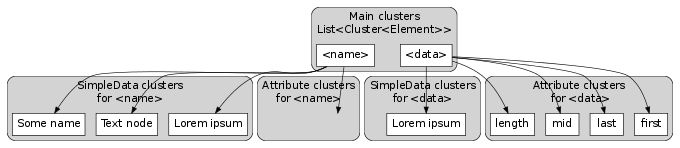
\includegraphics[scale=1]{clusterer_structure}
	\caption{Iname clusterer structure} \label{clusterer_structure}
\end{figure}

To rehearse, there are main clusters for elements, for each main cluster there are two helper clusterer - one for attribute clusters and one for simple data clusters.

%#### SUBMODULES->PassRepresentant ############################################
\subsection{PassRepresentant (ClusterProcessor)} \label{section_PassRepresentant}
Simple example to read. For each cluster return its representant as a rule to be in schema.
This has nothing to do with infering grammar, it is just proof of submodules concept.
Input documents are not valid against this odd grammar.
Do not use this in practice, just read the code to understand the bare minimum needed to implement submodule.

%#### SUBMODULES->Alternations ############################################
\subsection{Alternations (ClusterProcessor)} \label{section_Alternations}
This processor simply gets all right sides from elements in cluster, puts them in one big list and creates alternation regular expression with this list as children.
That is, it creates one big rule with alternation of every positive example observed.
No generalization is done at all.

%#### SUBMODULES->Trie ############################################
\subsection{Trie (ClusterProcessor)} \label{section_Trie}
This processor takes all rules in a cluster, treats them like strings and builds a prefix tree (a ``trie") of them. More precisely, it takes the first rule and declares it to be a long branch (concatenation of tokens) in a newly created tree. After that, it adds the remaining rules one by one as branches like this: as long as it can follow an existing branch, it follows it. As soon as the newly added branch starts to differ, it ``branches off" (creates an alternation at that point) the existing tree and hangs the rest of the newly added rule there. Repeating this process creates a prefix tree describing all the rules in the cluster.
The tree is the final regular expression.


%#### SUBMODULES->AutomatonMergingState ############################################
\subsection{AutomatonMergingState (ClusterProcessor)} \label{section_AutomatonMergingState}
\begin{figure}[tpb]
	\centering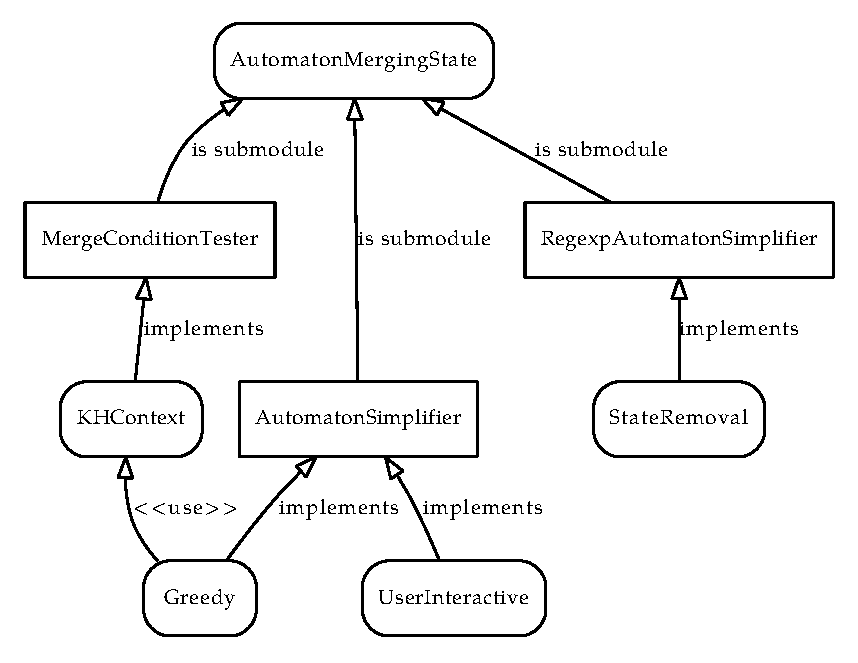
\includegraphics[scale=\myscale]{automaton_merging_state_modules}
	\caption{Submodules of AutomatonMergingState cluster processor} \label{automaton_merging_state_modules}
\end{figure}
\begin{figure}[tpb]
	\centering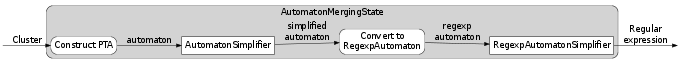
\includegraphics[scale=1]{automaton_merging_state_flow}
	\caption{Data flow of AutomatonMergingState cluster processor} \label{automaton_merging_state_flow}
\end{figure}
\jmodule{AutomatonMergingState} is implementation of merging state algorithm on nondeterministic finite automaton (see package \code{cz.cuni.mff.ksi.jinfer.twostep.processing.automatonmergingstate}).
\subsubsection{Structure} \label{section_AutomatonMergingState_structure}
Shortened code of cluster processor operation:
\begin{verbatim}
// 1. Construct PTA
final Automaton<AbstractStructuralNode> automaton = new Automaton<AbstractStructuralNode>(true);

// Take each rule in cluster and pass right side to automaton to create PTA
for (AbstractStructuralNode instance : rules) {
  final Element element = (Element) instance;
  final Regexp<AbstractStructuralNode> rightSide = element.getSubnodes();

  final List<AbstractStructuralNode> rightSideTokens = rightSide.getTokens();

  final List<AbstractStructuralNode> symbolString = new LinkedList<AbstractStructuralNode>();
  for (AbstractStructuralNode token : rightSideTokens) {
    symbolString.add(clusterer.getRepresentantForItem(token));
  }
  automaton.buildPTAOnSymbol(symbolString);
}

// 2. Simplify automaton by merging states using automatonSimplifier
final Automaton<AbstractStructuralNode> simplifiedAutomaton =
    automatonSimplifier.simplify(automaton, elementSymbolToString);

// 3. Convert Automaton<AbstractStructuralNode> to RegexpAutomaton<AbstractStructuralNode>
final RegexpAutomaton<AbstractStructuralNode> regexpAutomaton =
    new RegexpAutomaton<AbstractStructuralNode>(simplifiedAutomaton);
// 4. Call regexpAutomatonSimplifier to obtain regular expression from regexpAutomaton
final Regexp<AbstractStructuralNode> regexp =
    regexpAutomatonSimplifier.simplify(regexpAutomaton, regexpAbstractToString);

// 5. Return element with regexp
return new Element(
      new ArrayList<String>(),
      rules.get(0).getName(),
      new HashMap<String, Object>(),
      regexp,
      new ArrayList<Attribute>()
      );
\end{verbatim}
The whole submodule structure is drawn on fig. \ref{automaton_merging_state_modules}.

\subsubsection{Data flow}
It works in steps:
\begin{enumerate}
	\item It creates prefix-tree automaton (PTA) from positive examples - right sides of rules given.
Then it calls its submodule called \jmodule{AutomatonSimplifier} to  modify PTA to some generalized 
automaton by merging states.
	\item Simplified automaton is then converted to an instance of \code{RegexpAutomaton} (see \ref{section_RegexpAutomaton}) by using clone constructor.
Regexp automaton is automaton with regular expression as symbol on transitions.
In automata theory, such automaton is called extended NFA.
Clone constructing is done by converting each symbol in source automaton to regexp token with that symbol as \code{content}.
	\item \code{RegexpAutomaton} is then passed into second submodule called \jmodule{RegexpAutomatonSimplifier}.
Its job is to derive regular expression from automaton, such that automaton and regular expression represents same language.
\end{enumerate}
The data flow is on fig. \ref{automaton_merging_state_flow}.

\subsubsection{Data structures - Automaton} \label{section_Automaton}
\begin{figure}[tpb]
	\centering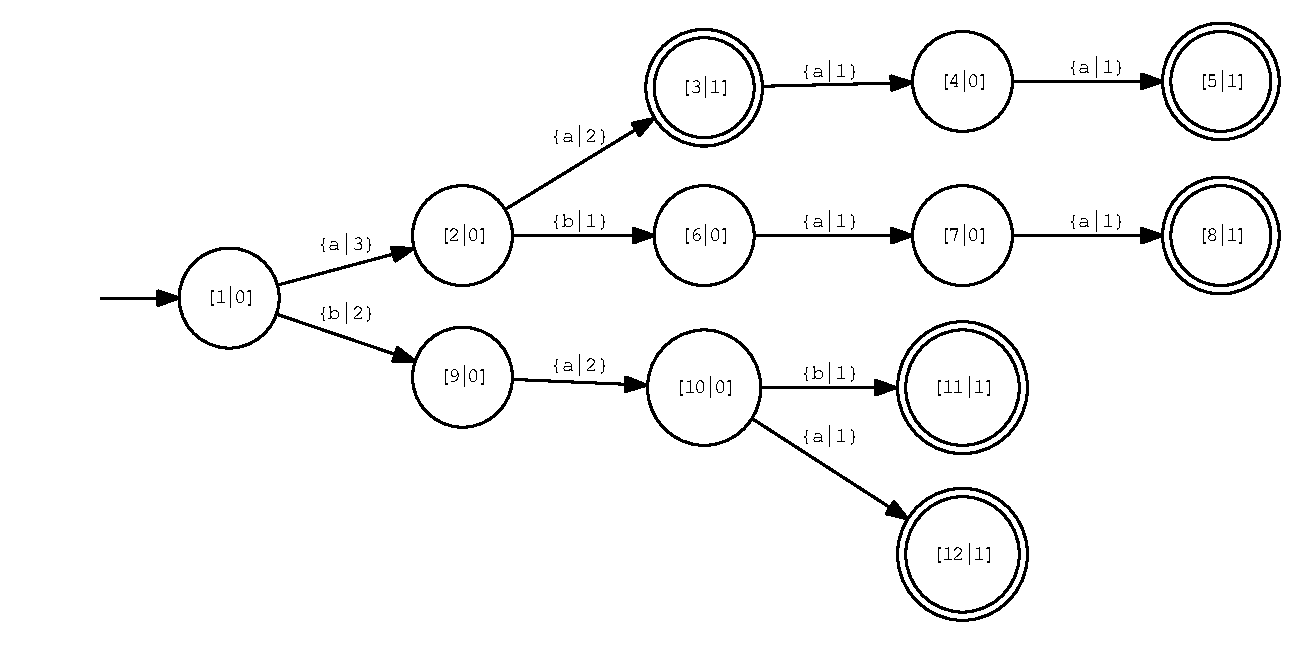
\includegraphics[scale=\myscale]{pta}
	\caption{PTA created from input strings: $aa, aaaaa, abaa, bab, baa$} \label{pta}
\end{figure}
Class \code{Automaton} is shortly described in \cite{archdoc}.
In this place, it is interestesting to look on method \code{build\.PTA\.On\.Sym\.bol}.
Given \code{List<T> symbolString} it traverses automaton - comparing transition symbols with symbols in string.
It follows transitions in automaton until first difference with string symbol is found (like in prefix trees).
On different symbol, it creates new branch and all states and transitions on that branch.
Last state visited got's incremented its \code{finalCount} value, as one more input string ended in this state.
Lets see code:
\begin{verbatim}
public void buildPTAOnSymbol(final List<T> symbolString) {
  State<T> xState= this.getInitialState();
  for (T symbol : symbolString) {
    final Step<T> xStep= this.getOutStepOnSymbol(xState, symbol);
    if (xStep != null) {
      xStep.incUseCount();
      xState= xStep.getDestination();
    } else {
      final State<T> newState= this.createNewState();
      final Step<T> newStep= this.createNewStep(symbol, xState, newState);
      assert newStep.getDestination().equals(newState);
      xState= newStep.getDestination();
    }
  }
  xState.incFinalCount();
}
\end{verbatim}
Start from initial state traverse automaton by asking for \code{getOutStepOnSymbol}.
If there is such step (transition), follow it to its destination state and move the position in \code{symbolString}.
If there is no such step, create one and create also the destination state, then follow this newly created step to new state.

As you can see, it is important that class \code{T} has proper implementation of \code{.equals()} method, as symbols are tested for equality by calling this method on them.
By the way, that is why we cluster all simple data and all sentinels on right sides of rules.
To automaton, instead of instances on right side of rules, their cluster representants are inserted as one can see in section \ref{section_AutomatonMergingState_structure}.
This assures, that comparisons in automaton are made by using java \code{Object.equals()} reference comparison, but for each cluster member, its representant is only present in automaton.
That results in cluster-equal behaviour.
Example of prefix-tree automaton is on fig. \ref{pta}.

\subsubsection{Data structures - RegexpAutomaton} \label{section_RegexpAutomaton}
Class \code{RegexpAutomaton} is extending class \code{Automaton} with generic type \code{T} set to \code{Regexp<T>}.
That is, you have to instantiate it with same symbol type (e.g. \code{AbstractStructuralNode}) as automaton.
Implementation can be found in package \code{cz.cuni.mff.ksi.jinfer.twostep.processing.automatonmergingstate.regexping}, that is same, as where \jmodule{RegexpAutomatonSimplifier} interface is defined.
Implementation is nothing special, it has only copy constructor which creates regular expression automaton from ordinary automaton by enclosing each symbol on transition of original automaton by \code{Regexp.TOKEN}.

\subsubsection{AutomatonSimplifier module}
\jmodule{AutomatonSimplifier} module has its worker interface defined as:
\begin{verbatim}
public interface AutomatonSimplifier<T> {
  Automaton<T> simplify(final Automaton<T> inputAutomaton, 
                        final SymbolToString<T> symbolToString) throws InterruptedException;
  Automaton<T> simplify(final Automaton<T> inputAutomaton, 
                        final SymbolToString<T> symbolToString,
                        final String elementName) throws InterruptedException;
}
\end{verbatim}
Given input automaton it returns automaton, there is nothing magical on it.
Interface is defined as generic, implementation don't have to be, but there is no reason to not make them generic.
When implementation needs to present automaton to user, however, it needs some string representation of symbols to display on automaton transitions.
For this reason, the second parameter, \code{symbolToString} (implementation of \code{SymbolToString} interaface) is given.
It is responsible for converting symbol to string.
To \jmodule{AutomatonSimplifier} it is passed from \jmodule{AutomatonMergingState} cluster processor, where we know that symbols are of type \code{AbstractStructuralNode}, so we implement \code{SymbolToString} by using \code{getName()} method on nodes and pass it down to generic \code{AutomatonSimplififier} submodule.
Overloaded version is to inform user about name of processed element when presenting automaton by \jmodule{AutoEditor}.
This version of interface will probably change in future.

By this genericity, simplifier can be used to perfom same algorithms for simplifying not only to infer rules for elements, but maybe also to infer patterns strings for content model of attributes.
The actual implementation of this still waits for its developer to come.
Implementations of \jmodule{AutomatonSimplifier} are discussed in \ref{section_Greedy} and \ref{section_UserInteractive}.

\subsubsection{RegexpAutomatonSimplifier submodule}
Purpose of \jmodule{RegexpAutomatonSimplifier} is to obtain regular expression from given automaton.
Interface for doing this is thus simple:
\begin{verbatim}
public interface RegexpAutomatonSimplifier<T> {
  Regexp<T> simplify(final RegexpAutomaton<T> inputAutomaton, 
                     final SymbolToString<Regexp<T>> symbolToString) throws InterruptedException;
}
\end{verbatim}
Once again we are encountering \code{symbolToString} with same purpose as before, if submodule would need to present automaton to user
it has to be able to convert symbols of (at runtime) unknown type to strings.
Our implementation of \jmodule{RegexpAutomatonSimplifier} is discussed in \ref{section_StateRemoval}

\subsubsection{MergeConditionTester submodule}
\jmodule{AutomatonMergingState} has one more submodule, the \jmodule{MergeConditionTester}, which is not called directly by \jmodule{Au\.to\.ma\.ton\.Merg\.ing\.Sta\.te}.
It is at disposal for implementations of \code{AutomatonSimplifier} interface for testing, whether two states in automaton are equivalent and should be merged into one state.

Module \jmodule{AutomatonSimplifier} implements solution searching logic in simplifying automaton by merging states.
One can implement ACO heuristics or MDL principle heuristics as \jmodule{AutomatonSimplifier} submodule, and can use any of \jmodule{MergeConditionTesters} provided.

\subsection{NestedConcatention (RegularExpressionCleaner)} \label{section_NestedConcatention}
This cleaner does exactly what we have just described.
It converts nested concatenations into flat ones.
Example: $(name, (person, id))$ is converted to $(name, person, id)$.

\subsection{Null (RegularExpressionCleaner)} \label{section_Null}
This cleaner just returns regexp it receives and does nothing.
Plug this one into chain, if you want to omit this step in inference.

\subsection{EmptyChildren (RegularExpressionCleaner)} \label{section_EmptyChildren}
Wipes out regular expressions of type: concatenation, alternation, permutation, which have empty \code{children} member.
For example some pitty inferring method produces unnecessary empty regexps in regexp tree as:
$$
(name, (), (person, id))
$$
There is one empty concatenation/alternation/permutation with no sense.
This is wiped out by this cleaner to produce 
$$
(name, (person, id))
$$

\subsection{Chained (RegularExpressionCleaner)} \label{section_Chained}
Enables user to chain more cleaners with output from first one plugged as input into second one and so one.
Thus regular expression from inference can pass through \jmodule{EmptyChildren} and them through \jmodule{NestedConcatenation} cleaners and then it is returned.

\subsection{Greedy (AutomatonSimplifier)} \label{section_Greedy}
We implement greedy strategy of automaton simplifying in class \code{Greedy}.
It simply asks given \code{MergeConditionTester} if it can merge any of automaton states and merges states until there are no states to be merged:
\begin{verbatim}
while (there exist pair of states that are equivalent) {
  merge them
}
\end{verbatim}
We provide one \jmodule{MergeConditionTester} implementation, see \ref{section_KHContext}.

\subsection{UserInteractive (AutomatonSimplifier)} \label{section_UserInteractive}
We have created automaton simplifier which displays user input automaton asking him to select some states to merge.
Then it merges them and asks user again:
\begin{verbatim}
repeat {
  draw automaton
  if (user selects more than one state to merge) {
    merge them
  }
} until (user selected at least one state in last trial)
\end{verbatim}
We use \jmodule{AutoEditor} module described in \cite{autoeditordoc}.
To make reader more happy, we include one screenshot of automaton visualization on picture \ref{screenshot}.
\begin{figure}[tpb]
	\centering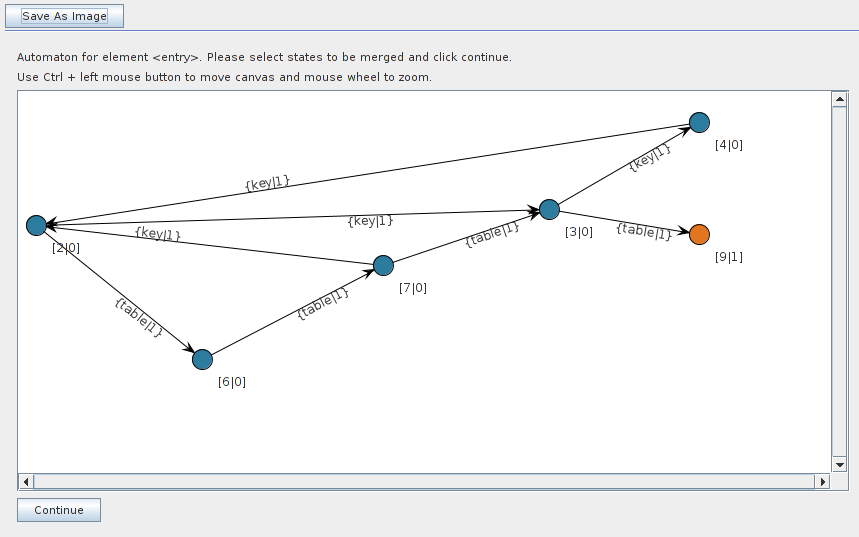
\includegraphics[scale=0.5]{screenshot}
	\caption{Screenshot of UserInteractive (AutomatonSimplifier).} \label{screenshot}
\end{figure}

\subsection{KHContext (MergeConditionTester)} \label{section_KHContext}
We have implemented \emph{k,h-context} state equivalence (see \cite{ahonen}) in class \code{KHContext} (implements \code{Mer\.ge\.Con\.di\.tion\.Tes\.ter} interface), which is used by \code{Greedy} to test mergability of states by default configuration.
TODO vektor : mention this? (we have stupid algorithm:)
We don't use $k-grams$ algorithm from \cite{ahonen}, but a simple DFS.

\subsection{StateRemoval (RegexpAutomatonSimplifier)} \label{section_StateRemoval}
\begin{wrapfigure}{R}{40mm}
	\centering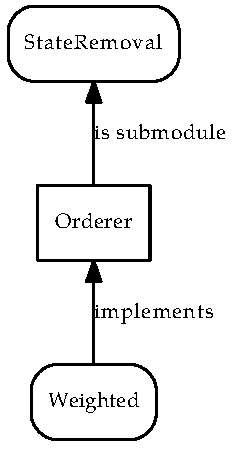
\includegraphics[scale=\myscale]{state_removal_modules}
	\caption{Modules of StateRemoval.} \label{state_removal_modules}
	\vspace{10mm}
\end{wrapfigure}
We are using state removal method (see \cite{1224321}) to convert regexp automaton into equivalent regular expression.
This is implemented in \code{StateRemoval} class (on fig. \ref{state_removal_modules}) which implements \code{RegexpAutomatonSimplifier} interface.
before algorithm starts, states superInitial and superFinal are added to automaton, former one with $\lambda$-transition to initial state.
From all final states $\lambda$ transition to superFinal state is added.
State removal works by removing states of automaton (and redirecting transitions properly) until there are last to two states - superInitial and superFinal.
After removing all states, there is only one transition from superInitial to superFinal state.
That transition has final regular expression on it as symbol, it is read and returned.

We defined one submodule of this class with \jmodule{Orderer}.
It has only one method to implement: \code{getStateToRemove}.
Given automaton, it has to return reference to one state which should be removed from automaton at first.
State removal calls this submodule and removes state returned.

\subsubsection{Data Structures - StateRemovalRegexpAutomaton}
We extend \code{RegexpAutomaton} to obtain automaton that fits state removing procedure.
This implementation has methods \code{crea\.te\.Su\.per\.In\.it\.ial\.Sta\.te} and \code{crea\.te\.Su\.per\.In\.it\.ial\.Sta\.te}.
They does exactly what their names stands for.
SuperInitial state has only one $\lambda$-out-transition pointing to original initial state.
SuperFinal state has as many $\lambda$-in-transitions, as there are original final states - from each one, it gets one.
Without going further to many technical details, we just mention method \code{removeState}, which removes given state from automaton.
Transitions are handled this way:
\begin{enumerate}
	\item Collapse all loop transition of removed state to one loop transition with new \code{Regex.ALTERNATION} of all regexps on original loops (with Kleene interval set).
	\item Collapse all {in | out}-transitions, which same {source | destination} state to one transition with \code{Reg\.exp.AL\.TER\.NA\.TION} of original regexps.
	\item For each in-transition, loop, and out-transition, add transition from in-transition source to out-transition destination with symbol of \code{Regexp.CONCATENATION} of in-transition regexp, loop regexp and out-transition regexp. Thus by-passing the state completely.
	\item Remove the state and transitions associated with it.
\end{enumerate}
Whole process is step-by-step illustrated on fig. \ref{regaut}.
\begin{figure}[pb]
	\centering
	\subfigure[RegexpAutomaton after conversion from ordinary automaton.]
	{
		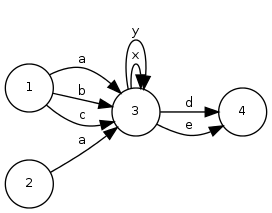
\includegraphics[scale=\myscale]{regaut1}
		\label{regaut1}
	}
	\subfigure[First, collapse loop transitions to alternation with Kleene interval set.]
	{
		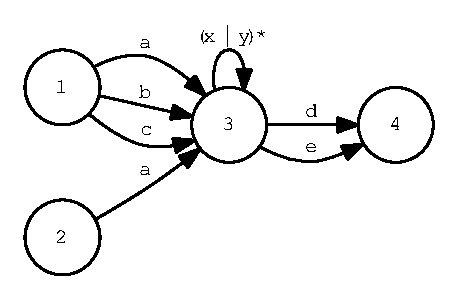
\includegraphics[scale=\myscale]{regaut2}
		\label{regaut2}
	}
	\subfigure[Collapse {in | out}-transitions {from | to} same states.]
	{
		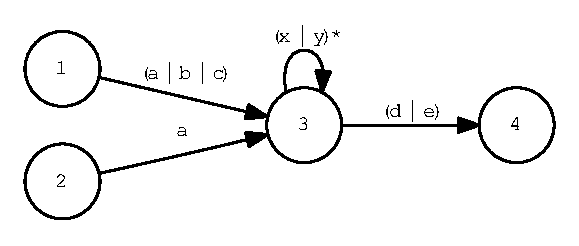
\includegraphics[scale=\myscale]{regaut3}
		\label{regaut3}
	}
	\subfigure[Bypass state 3 by adding concatenation transitions from states 1 and 2 to state 4. Remove state 3 and associated transitions.]
	{
		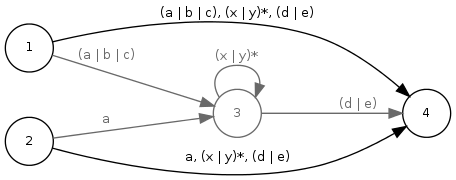
\includegraphics[scale=\myscale]{regaut4}
		\label{regaut4}
	}
%	
%	\subfigure[Finally remove state 3 and associated transitions.]
%	{
%		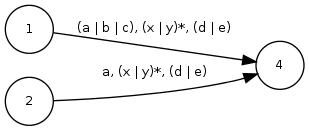
\includegraphics[scale=\myscale]{regaut5}
%		\label{regaut5}
%	}
	\caption{RegexpAutomaton and removing state 3 from it.} \label{regaut}
\end{figure}

\subsection{Weighted (Orderer)} \label{section_Weighted}
We implement one orderer, called \code{Weighted}.
It is simple heuristic - weights all states (weight = sum of {in | out | loop}-transition regular expression lengths) and returns state with lowest weight.

%#### EXTENSIBILITY ############################################
\section{Extensibility}
If you are willing to, you can replace each of three submodules of \jmodule{TwoStepSimplifier}.
It may be useful to replace default \jmodule{ClustererWithAttributes} implementation to a clever one.
And regular expression cleaning will be probably target of adding new implementations, too.
We recommend replacing other parts at lower levels, however.
You will need to replace \jmodule{ClusterProcessor} only if you want to write infering method that is not based on merging state algorithm (or NFA's at all).

If this is not your case, you can replace module \jmodule{AutomatonSimplifier} to implement ACO heuristics or MDL principle in searching solutions of merging states.

Of course, merge criterion is propably the point to add implementation, implement \jmodule{MergeConditionTester} interface to obtain for example $s,k$-string merge criterion.

Changing ordering of states to remove in \jmodule{StateRemoval} module is easy by replacing \jmodule{Orderer} implementation, for example to one of suggested in \cite{1224321} may lead to shorter resulting regular expressions.

Whole TwoStep submodules structure is on fig. \ref{twostep_modules_complete}.
\begin{figure}[tpb]
	\centering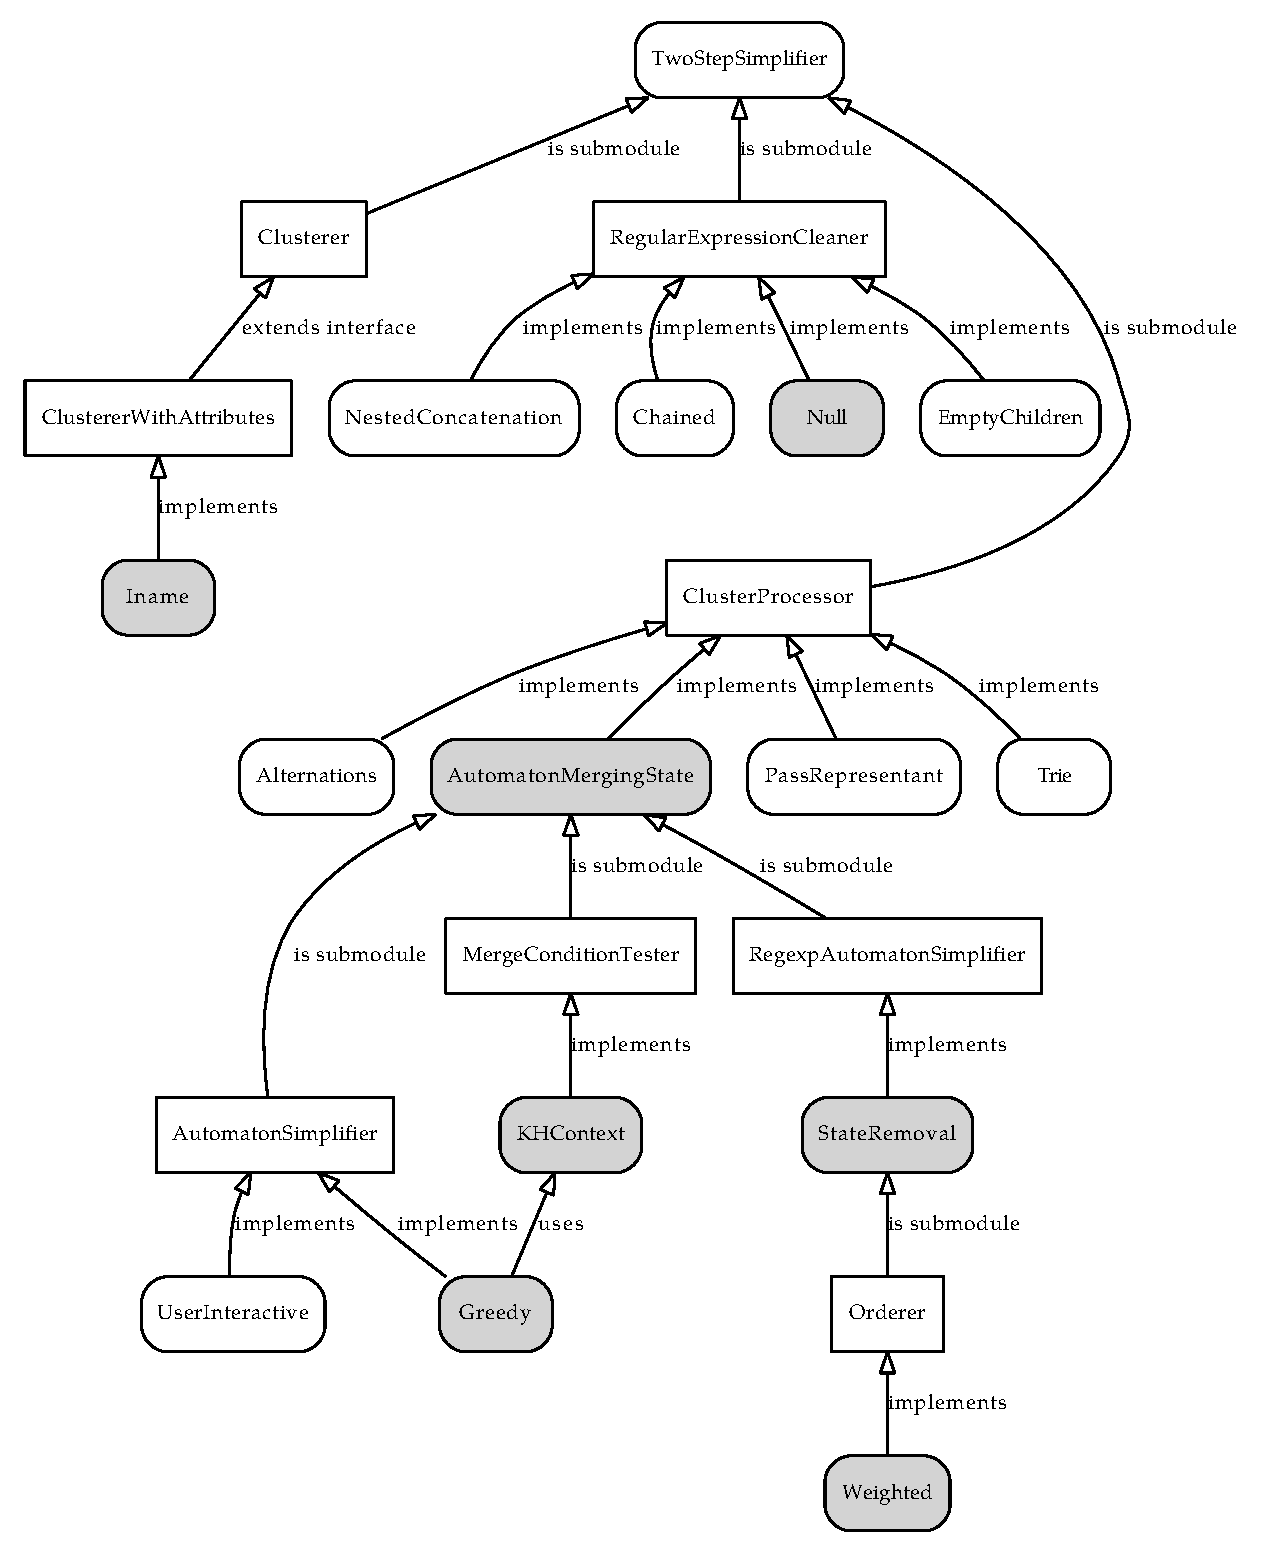
\includegraphics[scale=0.37]{twostep_modules_complete}
	\caption{Modules of TwoStep simplifier and their submodules. Filled classes are default selection (best of).} \label{twostep_modules_complete}
\end{figure}

\nocite{*}
\newpage
\bibliographystyle{alpha}
\bibliography{literature}

\end{document}
